\subsection{Spontaneous subduction}\label{sec:subduction}
This experiment is performed as presented by \citet{Schmeling2008}, in case of both a sticky air and a true free surface and using different average schemes
for the viscosities. The domain is rectangular with $L_x=$ \SI{3000}{\km} and $L_y=$ \SI{700}{\km}, a grid resolution of $256\times64$ elements with 50 markers
per element and Courant number of 0.01. At the beginning of the simulation, a 100 km-thick lithospheric layer with $\rho_m=$ \SI{3300}{\kg\per\cubic\metre}
and $\eta_m=$ \SI{e23}{\pascal\s} is located at the top of the domain for $x$ between 1000 and 3000 km, while the asthenospheric mantle has $\rho_m=$
\SI{3200}{\pascal\s} and $\eta_m=$ \SI{e21}{\pascal\s}. In addition, a 200 km-depth lithospheric slab is already subducted in the mantle in order to have
a spontaneous subduction. In case of sticky air, $L_y=750$ km and a 50 km-thick air layer with $\eta_a$ from \SIrange{e19}{e21}{\pascal\s} overlie the mantle.
Velocity boundary conditions are set to free slip on the sides and on the bottom of the domain. In case of sticky air, velocities on the top boundary are set
to free slip conditions as well.

\begin{wrapfigure}{r}{12cm}
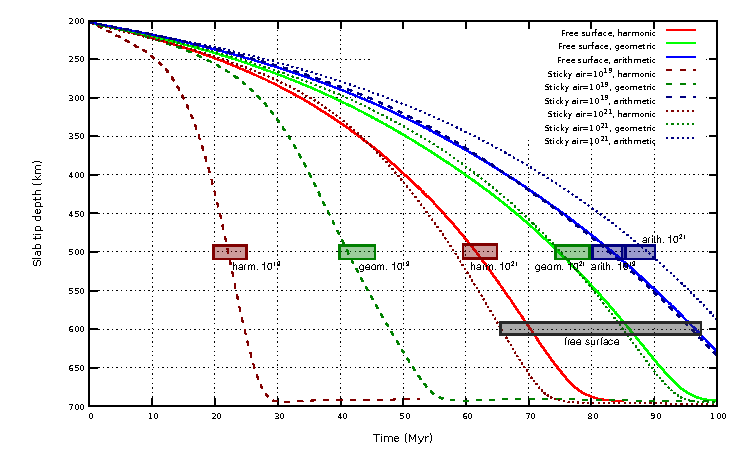
\includegraphics[width=12cm]{./Figures/Subduction.pdf}
\caption{Maximum depth of the slab as function of time for all the simulations of the \citet{Schmeling2008} benchmark, in case of harmonic, geometric and
arithmetic means (red, green and blue lines, respectively) using a sticky air or a true free surface (discontinuous and continuous lines, respectively).
Red, green and blue rectangular areas indicate the range of times from \citet{Schmeling2008} when the slab tip reaches \SI{500}{\km} in case of sticky air,
while the grey rectangular area indicates the range of times from \citet{Schmeling2008} when the slab tip reaches \SI{600}{\km} in case of true free surface.}
\label{fig:subduction}
\end{wrapfigure}
The maximum depth of the slab is tracked for all the simulations (Fig. \ref{fig:subduction}) and they are compared with results obtained by
\citet{Schmeling2008} with models with regular grids and comparable grid resolutions (rectangles in Fig. \ref{fig:subduction}). Low viscous sticky air models
(i.e., \SI{e19}{\pascal\s}) enlighten a strong dependence of the sinking velocity with the chosen average scheme (dashed lines in Fig. \ref{fig:subduction}),
while high viscous sticky air models (i.e., \SI{e21}{\pascal\s}) show a higher resistance at the trench, underestimating the correct solution (dotted lines in
Fig. \ref{fig:subduction}). A high resistance at the trench can be also observed in case of a true free surface for the low resolution grid used (continuous
lines in Fig. \ref{fig:subduction}), as pointed out by \citet{Schmeling2008}. All data can be 
found at \url{https://github.com/aleregorda/Benchmarks/tree/main/Surface_processes/Spontaneous_subduction}.